\chapter{类和对象}

\section{自定义类型}
\label{point}

\index{user-defined type 自定义类型}
\index{type!user-defined}

我们已经使用了很多Python的内置数据类型;现在我们将要定义自己的数据类型。
作为一个例子,我们将要创建一个{\tt Point}类型,代表二维空间的一个点。

\index{point ,mathematical 点,数学}

在数学记法中,点通常用写在括号里的坐标表示,中间用逗号隔开。比如,
$(0,0)$代表原点,$(x,y)$代表距离原点右边为$x$,上面为$y$的点。


在Python中,我们有多种表示点的方式。

\begin{itemize}

\item 我们可以把两个坐标存储在两个变量里,{\tt x}和{\tt y}.

\item 我们可把坐标存储在列表或者元组里。

\item 我们可以创建新的数据类类型来代表点。

\end{itemize}

\index{representation 代表}

创建型的数据类型相比于其他的方式来说有些许困难,但是优势也即将显现。

用户\footnote{译注:这里的用户指的是程序员,而不是终极用户。一般情况下用户的意思可以通过上下文来辨别。}自定义类型也叫做类。类的定义是这样:

\index{class 类}
\index{object 对象}
\index{class definition 类定义}
\index{definition!class}
\beforeverb
\begin{verbatim}
class Point(object):
    """represents a point in 2-D space"""
\end{verbatim}
\afterverb
%

类头表明新的类是{\tt Point},它也是一种对象。对象也是一种内置的数据类型。

\index{Point class Point类}
\index{class!Point}

类体是文档字符串(docstring),解释了{\tt Point}类的作用。我们可以在类
里定义变量和函数,我们一会儿就会涉及到。

\index{docstring 文档字符串}

定义一个{\tt Point}类,也就创建了一个类对象\footnote{译注:class object, 类对象,不是类的对象}。

\beforeverb
\begin{verbatim}
>>> print Point
<class '__main__.Point'>
\end{verbatim}
\afterverb
%

因为{\tt Point}是在顶级定义的,他的“全名”是\verb"__main__"。

\index{object!class}
\index{class object 类对象}


类对象就像是“制造”对象的工厂。为了创建一个类,我们可以像函数一样调用
{\tt Point}。

\beforeverb
\begin{verbatim}
>>> blank = Point()
>>> print blank
<__main__.Point instance at 0xb7e9d3ac>
\end{verbatim}
\afterverb
%

返回值是一个Point对象的引用,我们把它赋给{\tt blank}变量。创建一个新的对象叫实例化,对象是类的一个实例。

\index{instance 实例}
\index{instantiation 实例化}

当打印一个对象,Python告诉我们它是属于哪个类的,还有它存储的内存地址
(前缀{\tt ox} 表示后面的数字是十六进制的)。

\index{hexadecimal 十六进制}

\section{属性}

\index{instance attribute 实例属性}
\index{attribute!instance}
\index{dot notation 点记法}

我们可以使用点记法实例赋值。

\beforeverb
\begin{verbatim}
>>> blank.x = 3.0
>>> blank.y = 4.0
\end{verbatim}
\afterverb
%

 使用的语法和从模块里选择一个变量类似,就像{\tt math.pi}或者{\tt string.whitespace}。这里,我们给实例的元素赋值。这些元素叫做属性。

 作为一个名词,"AT-trib-ute"的第一个音节要发重音,和作为动词时“a-TRIB-ute,"相反。

 下面的图表显示了赋值后的结果。显示对象及其属性的状态图乘坐对象图。

 \index{state diagram 状态图}
 \index{diagram!state}
 \index{object diagram 对象图}
 \index{diagram!object}

 \beforefig
\centerline{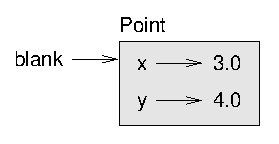
\includegraphics{figs/point.eps}}
\afterfig

{\tt blank}变量指向一个包含两个属性的点的对象。每一个属性指向一个浮点数。

我们可以通过同样的语法读取属性的值。

\beforeverb
\begin{verbatim}
>>> print blank.y
4.0
>>> x = blank.x
>>> print x
3.0
\end{verbatim}
\afterverb


表达式{\tt blank.x}意思是,“到{\tt blank}指向的对象去,获取{\tt x}的值。
此时,我们把取得的值赋给变量{\tt x}。变量{\tt x}和属性{\tt x}没有冲突。

我们可以在任何表达式中使用点记法。比如:

\beforeverb
\begin{verbatim}
>>> print '(%g, %g)' % (blank.x, blank.y)
(3.0, 4.0)
>>> distance = math.sqrt(blank.x**2 + blank.y**2)
>>> print distance
5.0
\end{verbatim}
\afterverb
%

也可以把一个实例作为参数传递。比如:

\index{instance!as argument}
\beforeverb
\begin{verbatim}
def print_point(p):
    print '(%g, %g)' % (p.x, p.y)
\end{verbatim}
\afterverb

\verb"print_point"接受一个点作为参数,并用数学记法显示它。我们可以把
{\tt blank}传递给它:

\beforeverb
\begin{verbatim}
>>> print_point(blank)
(3.0, 4.0)
\end{verbatim}
\afterverb
%

在函数里,{\tt p}是{\tt blank}的别名,所以如果函数改变了{\tt p},{\tt blank}也改变了\footnote{译注:Python中,只有引用}。

\index{aliasing 别名}

\begin{ex}
编写一个函数{\tt distance}接受两个点作为参数,返回两个点之间的距离。
\end{ex}



\section{矩形}

有时,很明显就可以看出对象需要什么属性,但是有时候,必须劳神费心一番。
比如,想象一下,你设计一个类来代表矩形。你会用什么属性来指定矩形的位置
和大小?忽略角度,也为了简单,假设举行是水平和竖直的。

\index{representation 代表}

至少有两种可能:

\begin{itemize}

\item 你可以指定矩形的一角(或者中心),宽度和高度。

\item 也可以指定对立的两个角。
\end{itemize}

此时,很难说明两种方式孰优孰劣。那我们就实现第一种把,仅仅作为一个例子.

\index{Rectangle class Rectangle类}
\index{class!Rectangle}

下面是一个类的定义:

\beforeverb
\begin{verbatim}
class Rectangle(object):
    """represent a rectangle. 
       attributes: width, height, corner.
    """
\end{verbatim}
\afterverb
%

文档字符串列举了所有的属性:{\tt width}和{\tt heigth}是数字,{\tt corner}是一个类的对象,代表了左下角。

为了代表一个矩形,我们必须实例化一个矩形的对象,给属性赋值:

\beforeverb
\begin{verbatim}
box = Rectangle()
box.width = 100.0
box.height = 200.0
box.corner = Point()
box.corner.x = 0.0
box.corner.y = 0.0
\end{verbatim}
\afterverb

表达式{\tt box.corner.x}意思是“到{\tt box}指向的对象那里,选择一个属性{\tt cornet};然后再到那个对象那里,选择{\tt x}属性。“

图表显示了对象的状态:

\index{state diagram 状态图}
\index{diagram!state}
\index{object diagram 对象图}
\index{diagram!object}

\beforefig
\centerline{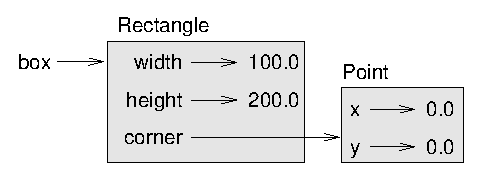
\includegraphics{figs/rectangle.eps}}
\afterfig
一个对象是另外一个对象的属性叫做嵌套。

\index{embeded object}
\index{object!embeded}

\section{实例作为返回值}

\index{instance!as return value}
\index{return value 返回值}

函数可以返回一个实例。比如,\verb"find_center"接受一个{\tt Rectangle}作为参数,返回包含{\tt Rectangle}中心点坐标的{\tt Point}。

beforeverb
\begin{verbatim}
def find_center(box):
    p = Point()
    p.x = box.corner.x + box.width/2.0
    p.y = box.corner.y + box.height/2.0
    return p
\end{verbatim}
\afterverb

下面是一个例子:把{\tt box}作为参数,把返回的点赋给变量{\tt center}:

\beforeverb
\begin{verbatim}
>>> center = find_center(box)
>>> print_point(center)
(50.0, 100.0)
\end{verbatim}
\afterverb
%

\section{对象是可变的}

\index{object!mutable}
\index{mutability 可变}

我们可以通过给对象的一个属性来改变对象的状态。比如,改变矩形的大小,但是不改变位置,我们可以修改{\tt width}和{\tt heigth}的值:

\beforeverb
\begin{verbatim}
box.width = box.width + 50
box.height = box.width + 100
\end{verbatim}
\afterverb
%

我们也可以编写函数来改变对象。比如,\verb"grow_rectangle"接受一个矩形对象,
和两个值,{\tt dwidth}和{\tt dheight},分别把{\tt dwidth}和{\tt dheight}
加到矩形的宽和高上:

\beforeverb
\begin{verbatim}
def grow_rectangle(rect, dwidth, dheight) :
    rect.width += dwidth
    rect.height += dheight
\end{verbatim}
\afterverb

下面的例子,演示了效果:

\beforeverb
\begin{verbatim}
>>> print box.width
100.0
>>> print box.height
200.0
>>> grow_rectangle(box, 50, 100)
>>> print box.width
150.0
>>> print box.height
300.0
\end{verbatim}
\afterverb

在函数体里,{\tt rect}是{\tt box}的别名,所以{\tt rect}改变时,{\tt box}也改变了。

\begin{ex}

编写一个函数\verb"move_rectangle"接受一个矩形和两个数字{\tt dx}和{\tt dy}。函数通过把{\tt dx}和{\tt dy}的值分别加到{\tt corner}点的{\tt x}和{\tt y}。
\end{ex}

\section{复制}

\index{aliasing 别名}

别名可以令程序难以阅读因为在一处改变了某些值可能会在其他某处产生不可预料的影响。很难跟踪所有指向给定对象的变量。

\index{copying objects 复制对象}
\index{object!copying}
\index{copy module copy模块}
\index{modue!copy}

选择复制对象是别名的一种替代方法。{\tt copy}模块包含了一个函数{\tt copy}
复制任意的对象:

\beforeverb
\begin{verbatim}
>>> p1 = Point()
>>> p1.x = 3.0
>>> p1.y = 4.0

>>> import copy
>>> p2 = copy.copy(p1)
\end{verbatim}
\afterverb

{\tt p1}和{\tt p2}包含了同样的数据,但是他们不是同一个点。

\beforeverb
\begin{verbatim}
>>> print_point(p1)
(3.0, 4.0)
>>> print_point(p2)
(3.0, 4.0)
>>> p1 is p2
False
>>> p1 == p2
False
\end{verbatim}
\afterverb

{\tt is}操作符表明{\tt p1}和{\tt p2}不是同一个对象,这是我们希望的。但
是你或许希望{\tt ==}运算符产生{\tt True},因为这两个点包含了同样的数据。
在这种情况下,你可能会失望的了解到对于实例,{\tt ==}缺省的行为和{\tt is}操作符是相同的;它检查对象的身份而不是对象数据是否相等。我们也可以
改变这种行为---我们不久就会看到。

\index{is operator is运算符}
\index{operator!is}

我们可以使用{\tt copy.copy}复制长方形,我们将发现它复制了矩形对象,但是没有复制嵌套的点。

\index{embeded object!copying}

\beforeverb
\begin{verbatim}
>>> box2 = copy.copy(box)
>>> box2 is box
False
>>> box2.corner is box.corner
True
\end{verbatim}
\afterverb

下面是对象图:

\index{state diagrm 状态图}
\index{diagram!state}
\index{object diagram 对象图}
\index{diagram!object}

\vspace{0.1in}
\beforefig
\centerline{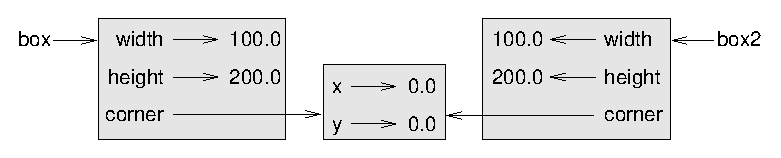
\includegraphics{figs/rectangle2.eps}}
\afterfig
\vspace{0.1in}

这种操作叫做浅拷贝,因为它拷贝了对象和它包含的引用,但是不包括嵌套的对象。

\index{shallow copy 浅拷贝}
\index{copy!shallow}

对于大多数的应用来说,这不是你想要的。此时,调用\verb"grow_rectangle"不会影响其他的其他的矩形。但是调用\verb"move_rectangle"会影响双方!这种
行为很容易令人迷惑,也很容易产生错误。

\index{deep copy 深拷贝}
\index{copy!deep}

幸运的是,{\tt copy}模括包含了另外一个方法{\tt deepcopy},不仅复制对象本身,也复制对象指向的东西及其指向的东西等等。

你讲不会对这种操作叫做深拷贝而惊讶。

\index{deepcopy function deepcopy 函数}
\index{function!deepcopy}

\beforeverb
\begin{verbatim}
>>> box3 = copy.deepcopy(box)
>>> box3 is box
False
>>> box3.corner is box.corner
False
\end{verbatim}
\afterverb
%

{\tt box3}和{\tt box}是两个完全分离的对象。

\begin{ex}
编写另外一种版本\verb"move_rectangle"创建并返回一个新的矩形,不要改变原来的矩形。
\end{ex}

\section{调试}
\label{hasattr}

\index{debugging 调试}

当使用对象的时候,我们很可能会遇到一些新的异常。如果你访问一个不存在的
属性,将会得到{\tt AttributeError}异常:

\index{exception!AttributeError}
\index{AttributeError}

\beforeverb
\begin{verbatim}
>>> p = Point()
>>> print p.z
AttributeError: Point instance has no attribute 'z'
\end{verbatim}
\afterverb

如果不能确定对象的类型是什么,可以这样:

\index{type function type函数}
\index{function!type}

\beforeverb
\begin{verbatim}
>>> type(p)
<type '__main__.Point'>
\end{verbatim}
\afterverb
%

如果不确定对象是否拥有一个属性,可以使用内置的函数{\tt hasattr}:

\beforeverb
\begin{verbatim}
>>> hasattr(p, 'x')
True
>>> hasattr(p, 'z')
False
\end{verbatim}
\afterverb
%

第一个参数可以是任意对象,第二个参数是一个字符串包含要查询的属性。

\section{术语表}

\begin{description}

\item [class 类:] 用户自定义类型。类的定义创建了一个类对象。
\index{class}

\item [class object 类对象:] 包含用户自定义类型信息的对象。类对象
可以用来产生一个实例。
\index{class object 类对象}

\item [instance 实例:]属于类的对象。
\index{instance 实例}

\item [attribute 属性:]一个和对象相关的命名的值。
\index{attribute!instance}
\index{instance attribute 实例属性}

\item [embededed (object) 嵌套对象:]作为属性存储在其他对象里的对象。
\index{embededed object 嵌套对象}
\index{object!embedded}

\item [shallow copy浅拷贝:]拷贝对象的结构,包括指向嵌套对象的引用;通过{\tt copy}模块的{\tt copy}函数实现。
\index{shallow copy}

\item [deep copy 深拷贝:]拷贝对象的结构嵌套对象和包含在嵌套对象里的对象,如此如此;通过{\tt copy}模块的{\tt deepcopy}函数实现。
\index{deep copy 深拷贝}

\item [object daigram 对象图:]显示对象及其书香和属性值的图表。
\index{object diagram 对象图}
\index{diagram!object}
\end{description}

\section{练习}

\begin{ex}
\label{canvas}

\index{Swampy}
\index{World module World模块}
\index{module!World}

Swampy(参看\ref{turtlechap})有一个模块,{\tt World.py},包含了自定义的类定义{\tt World}。你可以这样导入它:

\beforeverb
\begin{verbatim}
from World import World
\end{verbatim}
\afterverb

这个版本的{\tt import}语句从{\tt World}模块导入了{\tt World}类。下面的
代码创建了一个World 对象,并且调用了{\tt mainloop}方法,等待用户。

\beforeverb
\begin{verbatim}
world = World()
world.mainloop()
\end{verbatim}
\afterverb

应该出现了一个带有框和空白区域的窗口。我们将要使用这个窗口画点,长方形还有其他的图形。把下面的代码加到\verb"mainloop"的前面,运行这个程序。

\index{Canvas object}
\index{object!Canvas}

\beforeverb
\begin{verbatim}
canvas = world.ca(width=500, height=500, background='white')
bbox = [[-150,-100], [150, 100]]
canvas.rectangle(bbox, outline='black', width=2, fill='green4')
\end{verbatim}
\afterverb

你应该看到了一个边是黑色的绿色矩形,代码的第一行创建了一个画布,以空白区域填充窗口。画布对象提供了一些方法像{\tt rectangle}来绘制不同的图形。

\index{bounding box }

{\tt bbox}是序列表,代表了矩形的边界。第一个坐标对代表了矩形左下角,第二
个坐标代表了右上角。

你可以这么样来绘制一个圆:

\beforeverb
\begin{verbatim}
canvas.circle([-25,0], 70, outline=None, fill='red')
\end{verbatim}
\afterverb

\index{Bangladesh, national flag 孟加拉国,国旗}

第一个参数是圆心的坐标;第二个参数是半径。

如果把这条代码加入到程序中,将会看到类似孟加拉国国旗的图形。(参看\url{wikipedia.org/wiki/Gallery_of_sovereign-state_flags})。

\begin{enumerate}

\item 编写一个函数\verb"draw_rectangle",接受一个画布和矩形为参数,在画
布上绘制矩形。

\item 在你的矩形对象里增加一个{\tt color}属性,修改\verb"draw_rectangle" 使得用颜色属性作为填充颜色。

\item 编写一个函数\verb"draw_point",接受一个画布和点作为参数,在华布上画一个点。

\item 定义一个类{\tt Circle},自己定义适当的属性,实例化一些Circle对象。编写函数\verb"draw_cicle"在华布上画圆。

\index{Czech Republic, national flag 捷克共和国,国旗}

\item 编写一个程序绘制捷克共和国的国旗。Hint:可以这样绘制一个多边形:

\beforeverb
\begin{verbatim}
points = [[-150,-100], [150, 100], [150, -100]]
canvas.polygon(points, fill='blue')
\end{verbatim}
\afterverb

\end{enumerate}

\index{color list}
\index{available colors}

我已经编写了一些程序,列出了可供使用的颜色;可以从这儿下载\url{thinkpython.com/code/color_list.py}.
\end{ex}
















































































































































































